%-----------------------------------LICENSE------------------------------------%
%   This file is part of tikz_figures.                                         %
%                                                                              %
%   tikz_figures is free software: you can redistribute it and/or              %
%   modify it it under the terms of the GNU General Public License as          %
%   published by the Free Software Foundation, either version 3 of the         %
%   License, or (at your option) any later version.                            %
%                                                                              %
%   tikz_figures is distributed in the hope that it will be useful,            %
%   but WITHOUT ANY WARRANTY; without even the implied warranty of             %
%   MERCHANTABILITY or FITNESS FOR A PARTICULAR PURPOSE.  See the              %
%   GNU General Public License for more details.                               %
%                                                                              %
%   You should have received a copy of the GNU General Public License along    %
%   with tikz_figures.  If not, see <https://www.gnu.org/licenses/>.           %
%------------------------------------------------------------------------------%

% Use the standalone class for displaying the tikz image on a small PDF.
\documentclass[crop, tikz]{standalone}

% Import the tikz package to use for the drawing.
\usepackage{tikz}

% Tikz packages used.
\usetikzlibrary{decorations.markings}

% Begin the document.
\begin{document}

    % Draw the figure.
    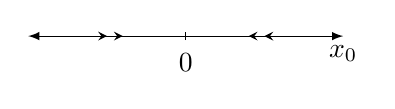
\begin{tikzpicture}

        % The entire phase line is drawn using the decoractions library.
        \draw[%
            shorten < = 0.5mm,
            shorten > = 0.5mm,
            postaction = {decorate},
            decoration = {%
                markings,
                mark = at position 0.00 with \arrowreversed{latex},
                mark = at position 0.25 with \arrow{stealth},
                mark = at position 0.30 with \arrow{stealth},
                mark = at position 0.50 with {%
                    \draw[thin] (0, -1mm) to (0, 1mm) node [below = 2mm] {0};
                },
                mark = at position 0.75 with \arrowreversed{stealth},
                mark = at position 0.70 with \arrowreversed{stealth},
                mark = at position 1.00 with \arrow{latex},
            },
        ] (-2.0, 0.0) to (2.0, 0.0) node[below] {$x_{0}$};
    \end{tikzpicture}
\end{document}
